\clearpage
\subsection{Scheduled excavation in three stages}
\label{sec:staged-excavation-example}

\subsubsection*{Geometry and material}

This example demonstrates three scheduled removals and the resulting large deformation. The domain is 475 m wide in X, 250 m high in Z, and 5 m thick in Y. Three rock regions arranged along an inclined band are removed successively, starting at the existing excavation floor.

The grid has $95\times1\times50$ cubic cells with side length 5 m. The rock is divided into six bodies: three permanent regions and three removable regions. All regions use the same Mohr--Coulomb parameters, listed in Table~\ref{tab:excavation-material}. The bodies share the grid field; no separate frictional material-contact condition is activated.

\begin{table}[H]
    \centering
    \caption{Material parameters used in both stages.}
    \label{tab:excavation-material}
    \begin{tabular}{lr}
        \toprule
        Parameter & Value \\
        \midrule
        Young's modulus & 20 GPa \\
        Poisson's ratio & 0.20 \\
        Density & 2700 kg/m$^3$ \\
        Cohesion & 0.5 MPa \\
        Friction angle & $20^\circ$ \\
        Dilation angle & $0^\circ$ \\
        Tensile strength & 0 Pa \\
        \bottomrule
    \end{tabular}
\end{table}

Gravity is $9.81$ m/s$^2$ in the negative Z direction. The base is fixed. The X and Y boundary planes prevent normal motion and allow tangential motion; the upper Z plane is free. Both stages use single-phase USL integration.

\begin{figure}[H]
    \centering
    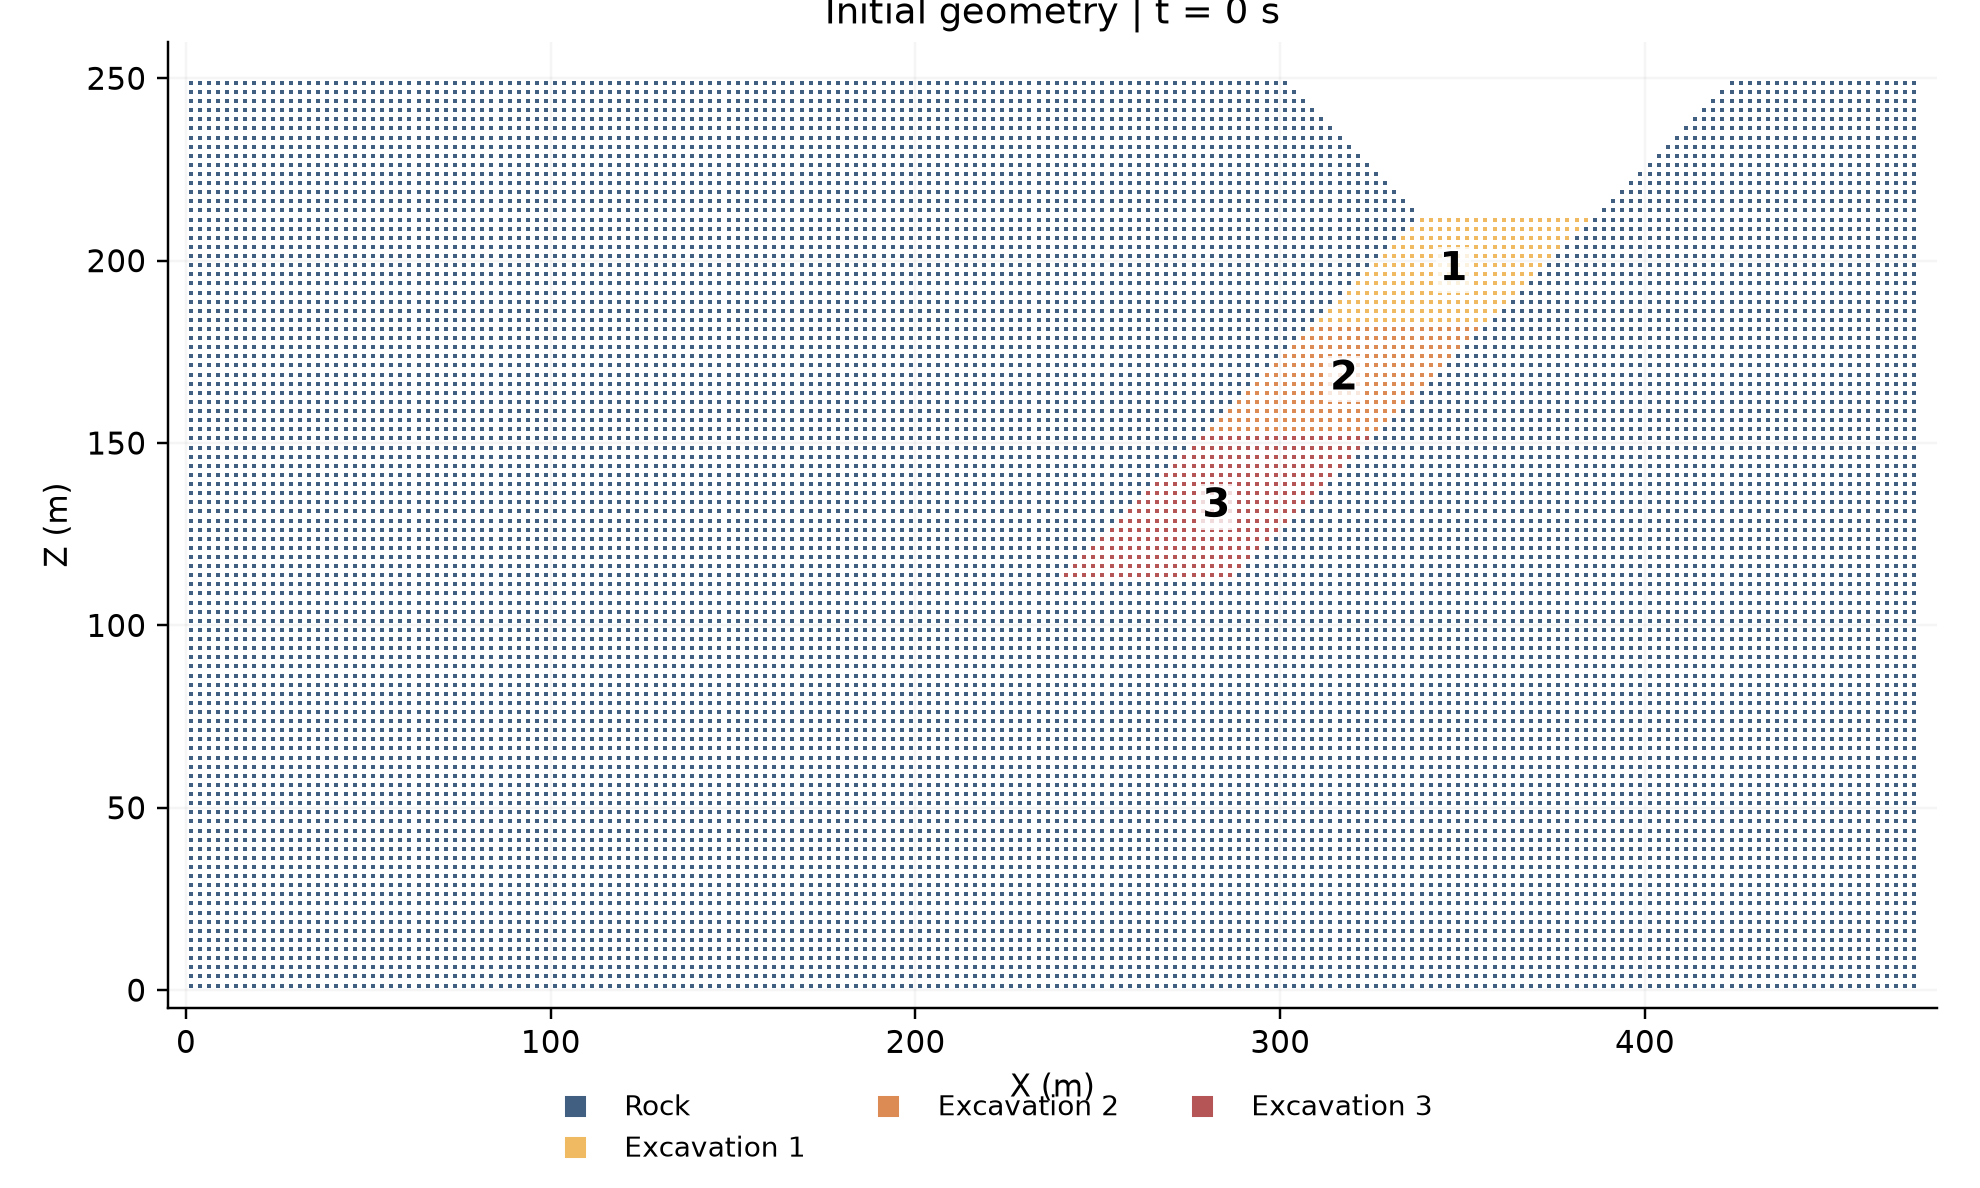
\includegraphics[width=0.95\textwidth]{figures/staged-excavation-initial.png}
    \caption{Initial geometry of the excavation stage. The three scheduled regions are identified by their removal order.}
    \label{fig:excavation-initial}
\end{figure}

\subsubsection*{Gravity initialization}

The first analysis applies the weight of the complete geometry for 1 s with kinetic damping and no scheduled removals. In the last saved output, the maximum particle speed is $1.60\times10^{-7}$ m/s and the kinetic energy is $2.25\times10^{-6}$ J. The maximum displacement is approximately 0.04115 m, and its change between the last two outputs is approximately $10^{-6}$ m at exported precision. These results indicate that the gravity initialization has settled.

The second analysis imports the resulting stress tensors. It recreates the original particle positions, and starts with zero velocitie. During the interval before the first removal, the maximum saved displacement is approximately $4.18\times10^{-5}$ m, showing a small residual adjustment to this transfer.

\subsubsection*{Input files}

The excavation schedule is defined by \texttt{excavation\_time} inside each removable body's definition. The three regions in this example are removed at 0.25, 0.5 and 2.5 s:
\begin{lstlisting}
"body": {
  "excavation_1": {
    "type": "particles",
    "particles": { ... },
    "excavation_time": 0.25
  },
  "excavation_2": {
    "type": "particles",
    "particles": { ... },
    "excavation_time": 0.5
  },
  "excavation_3": {
    "type": "particles",
    "particles": { ... },
    "excavation_time": 2.5
  }
}
\end{lstlisting}
This fragment omits the particle arrays and permanent bodies. The permanent bodies have no \texttt{excavation\_time} entry. The time in the excavation analysis starts at zero independently of the initialization analysis. The complete input imports the initialized stresses, disables damping and runs for 5 s.

\subsubsection*{Geometry before and after removal}

Figures~\ref{fig:excavation-event-1}--\ref{fig:excavation-event-3} compare the deformed particle positions immediately before and after each removal. The removal is evaluated at the start of the step. 


\begin{figure}[H]
    \centering
    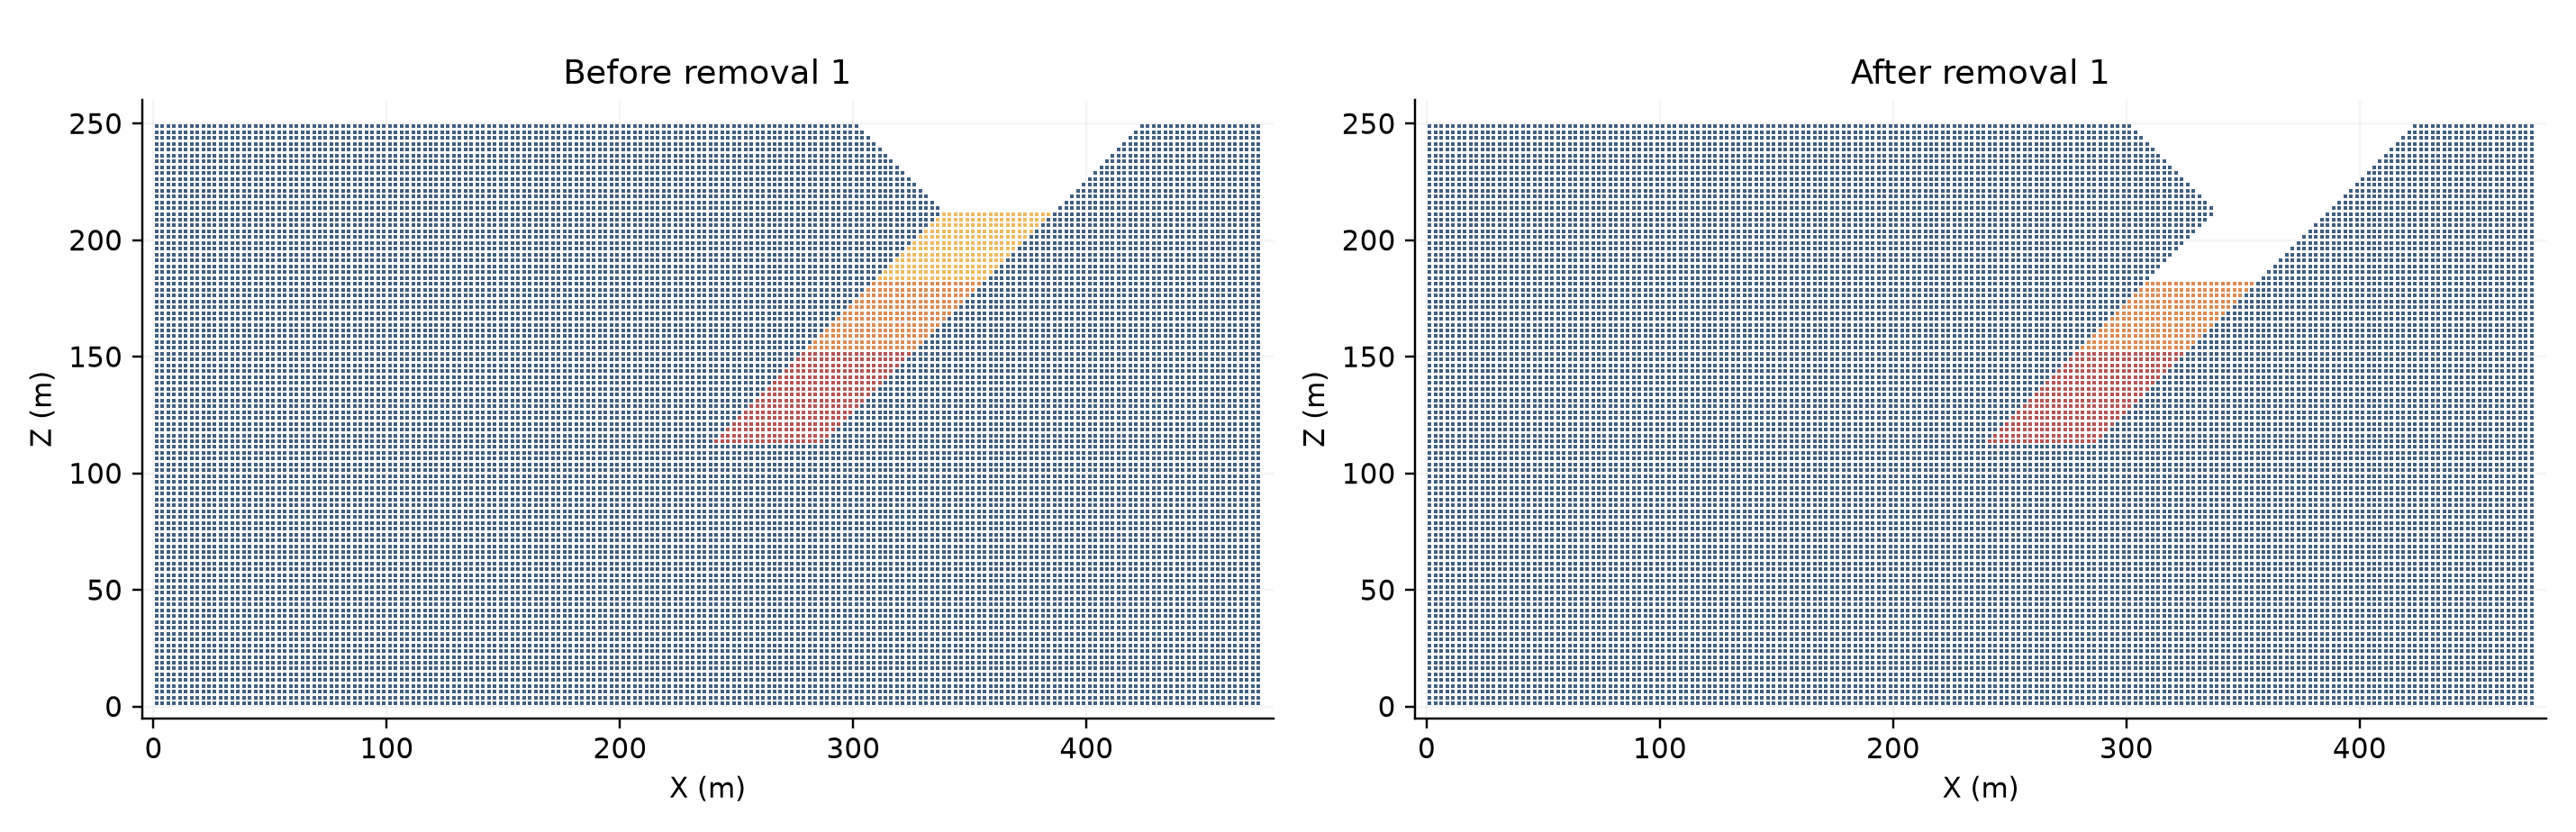
\includegraphics[width=\textwidth]{figures/staged-excavation-event-1.png}
    \caption{First excavation, scheduled at 0.25 s: adjacent states before and after removal, with inactive particles hidden.}
    \label{fig:excavation-event-1}
\end{figure}

\begin{figure}[H]
    \centering
    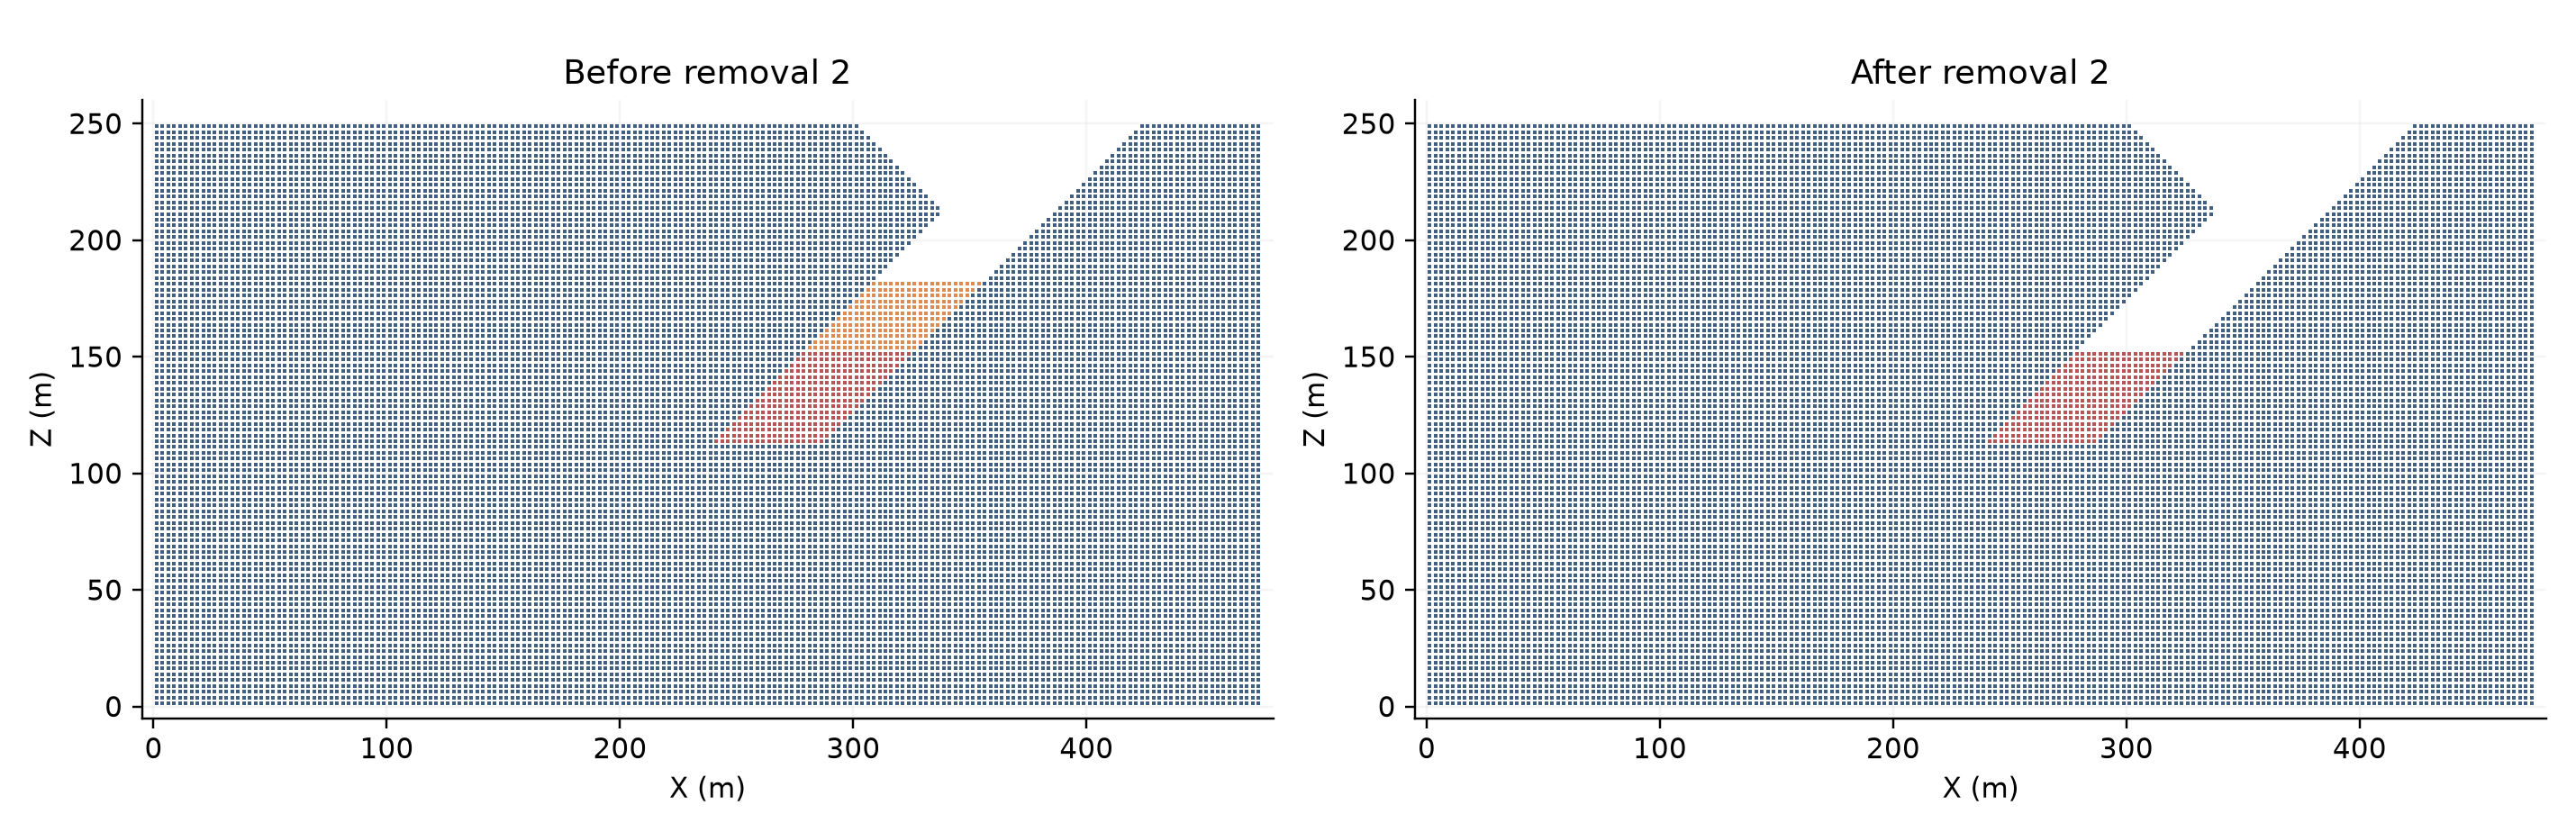
\includegraphics[width=\textwidth]{figures/staged-excavation-event-2.png}
    \caption{Second excavation, scheduled at 0.5 s: adjacent states before and after removal, with inactive particles hidden.}
    \label{fig:excavation-event-2}
\end{figure}

\begin{figure}[H]
    \centering
    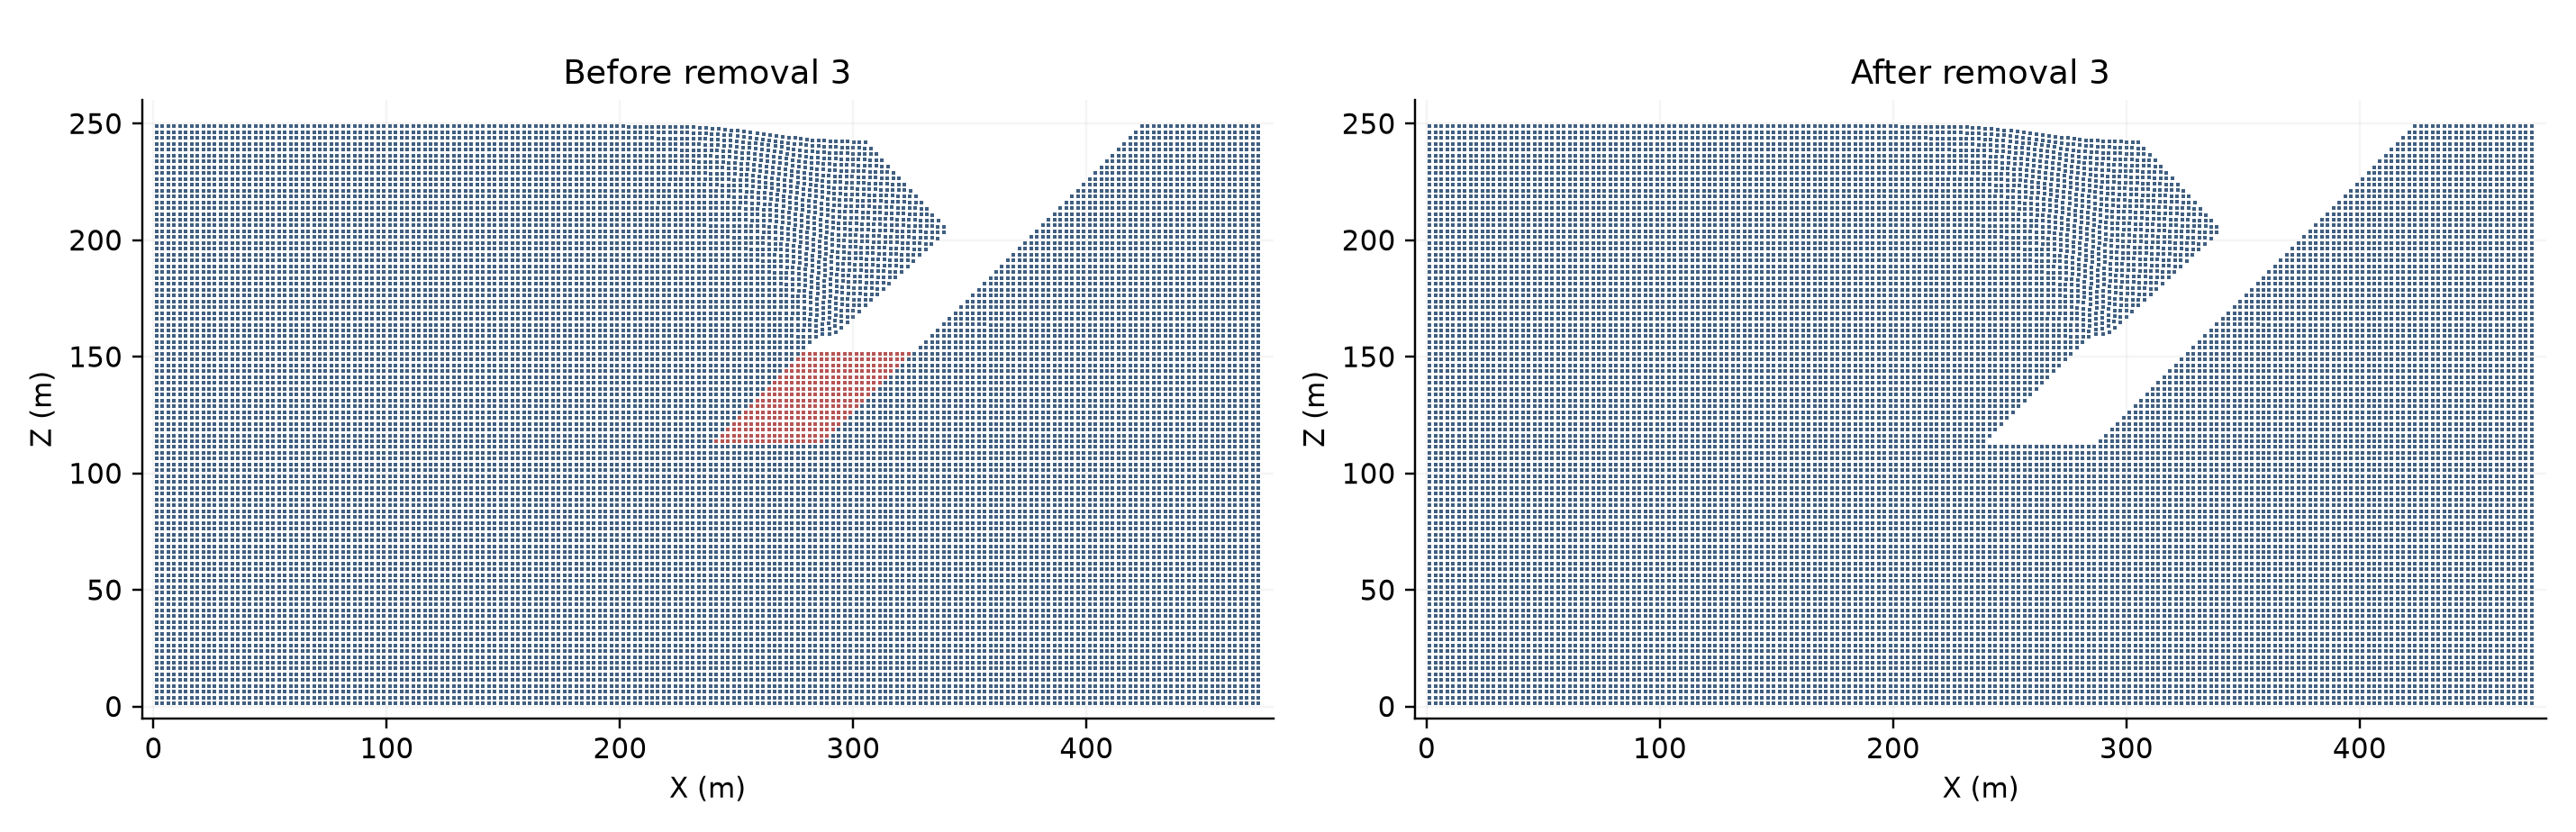
\includegraphics[width=\textwidth]{figures/staged-excavation-event-3.png}
    \caption{Third excavation, scheduled at 2.5 s: adjacent states before and after removal, with inactive particles hidden.}
    \label{fig:excavation-event-3}
\end{figure}

\subsubsection*{Geometry at the end of the analysis}

After the three removals, 35,460 particles remain active. The original 5 s run recorded a maximum displacement of 38.70 m. Figure~\ref{fig:excavation-final} shows the deformed geometry at the end of the excavation analysis. The example checks the timing and identity of removed bodies and illustrates the motion of the remaining material.

\begin{figure}[H]
    \centering
    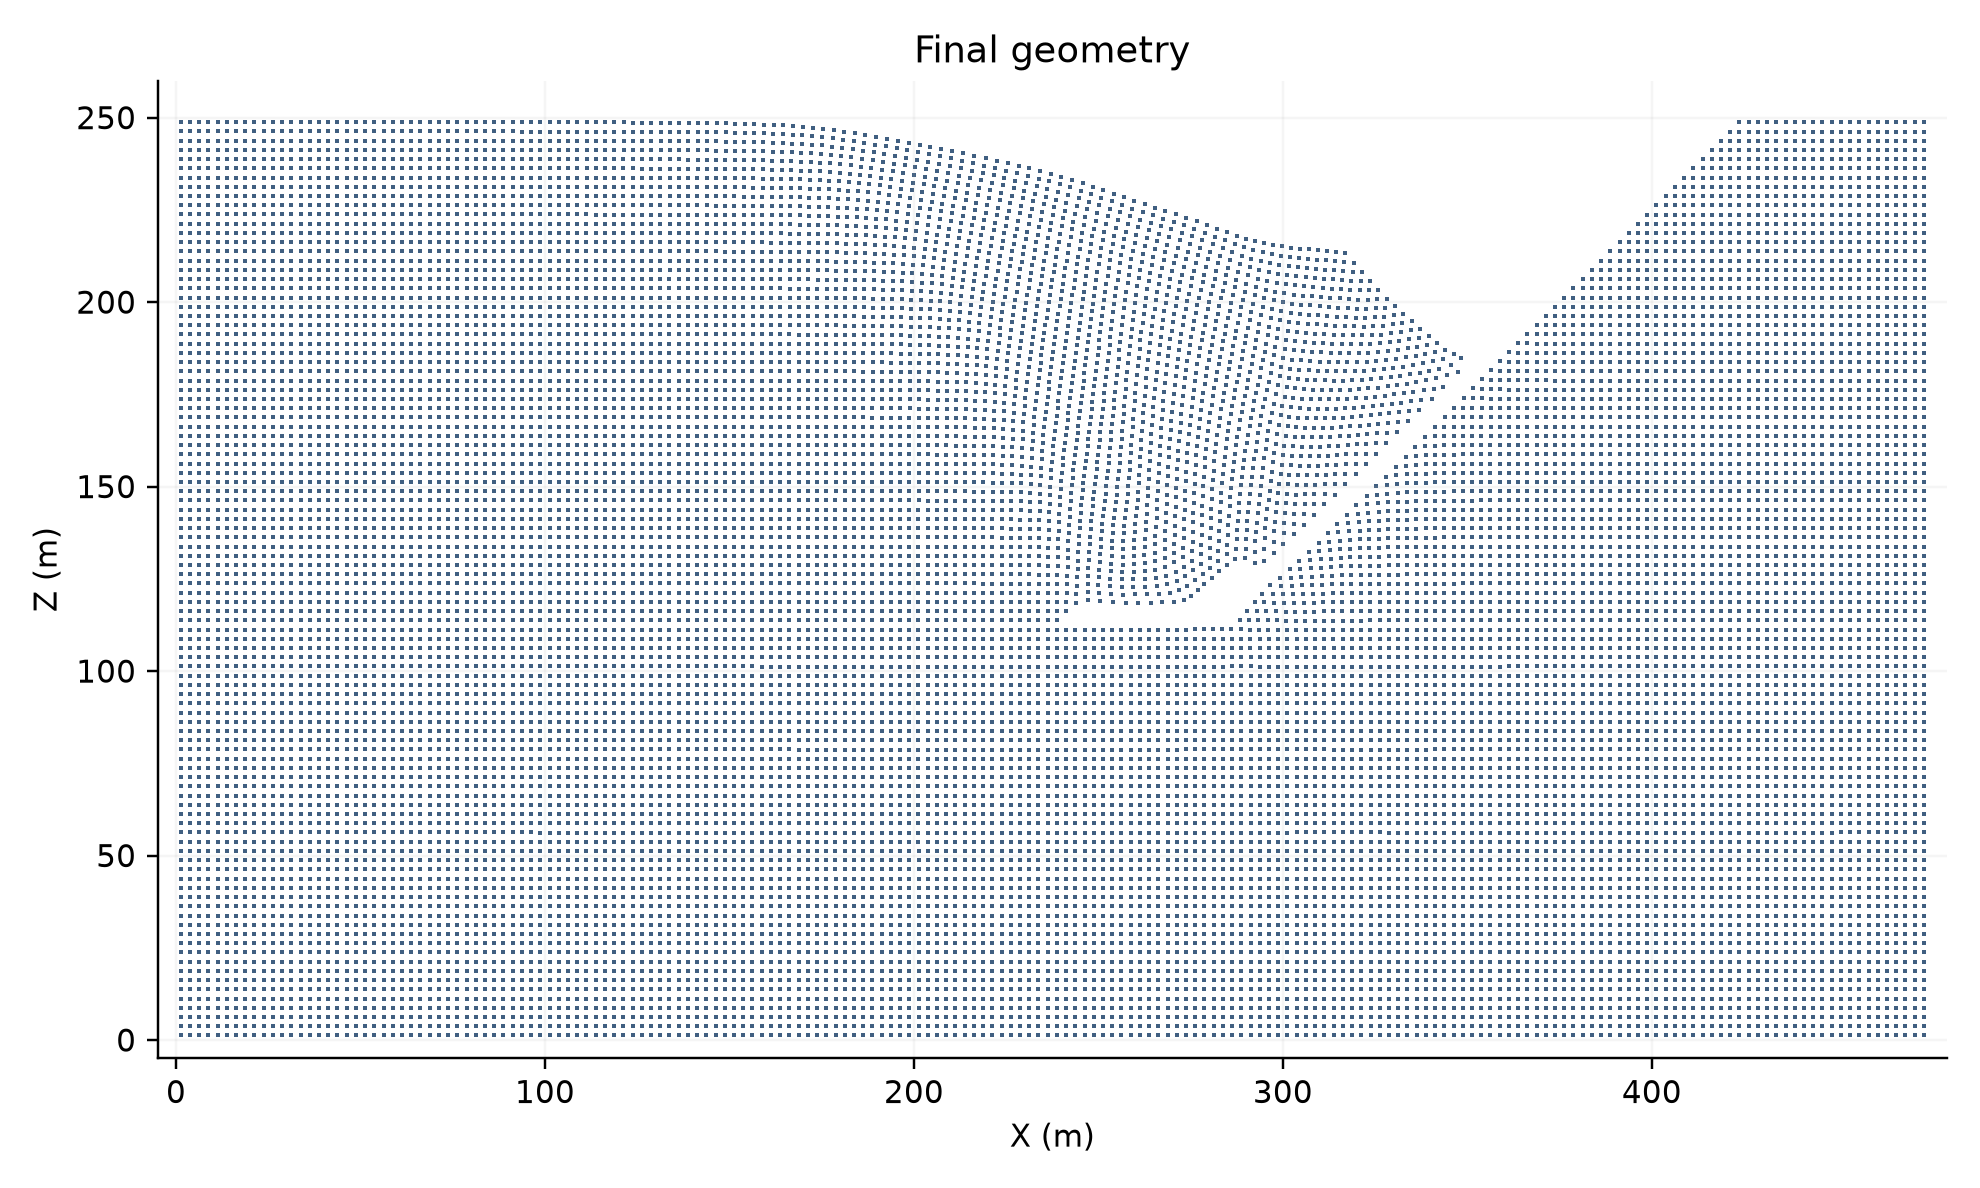
\includegraphics[width=0.95\textwidth]{figures/staged-excavation-final.png}
    \caption{Deformed geometry at the end of the excavation analysis.}
    \label{fig:excavation-final}
\end{figure}

